\begin{problem}%
{Маленькое новоселье}%
{\textsl{стандартный ввод}}%
{\textsl{стандартный вывод}}%
{1 секунда}%
{256 мегабайт}{}

Ситуация с землёй в столице одной малоизвестной страны приближается к катастрофической. Уже практически невозможно найти даже небольшой клочок земли для постройки своего жилища.
Тем не менее Фёдору повезло: после прохождения многочисленных инстанций он всё-таки нашел место для нового дома. Более того, щедрое правительство даже подарило ему невероятно красивую крышу для постройки.\\

Важным обстоятельством является то, что Федя — совершенно плоский, как и весь мир, который его окружает. В этом плоском мире введена стандартная декартова система координат: ось $O_x$ совпадает с землёй, а ось $O_y$ направлена от земли вверх. Крыша представляет собой два отрезка, исходящих из одной точки (вершины крыши) вниз в разные стороны, причём оба отрезка составляют угол 45 градусов с осью $O_x$:\\

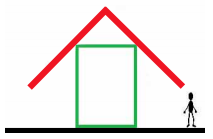
\includegraphics[]{images/1.png}

Разумеется, крыша находится над землёй, то есть отрезки находятся в верхней полуплоскости. Оба отрезка имеют ненулевую длину. Дом Феди должен представлять собой прямоугольник со сторонами, параллельными осям координат, одна сторона которого находится на земле, а другая сторона упирается в оба отрезка крыши. Дом не должен выходить за пределы крыши по горизонтали. Помогите Феде построить для себя дом наибольшей площади.

\InputFile

В первой строке содержатся два целых числа $x_c$ и $y_c$ — координаты вершины крыши ($\abs{x_c} \le 10^4$, $1 \le y_c \le 10^4$).\\

Во второй строке содержатся два целых числа $x_1$ и $y_1$ — координаты одного из концов крыши ($\abs{x_1} \le 10^4$, $x_1 \ne x_c$, $0 \le y_1 < y_c$). В следующей строке в таком же формате заданы координаты $x_2$ и $y_2$ другого конца крыши.\\

Гарантируется, что отрезки, образующие крышу, направлены в разные стороны относительно верхней точки крыши, т.е. либо $x_1$ < $x_c$ < $x_2$, либо $x_2$ < $x_c$ < $x_1$, оба отрезка имеют одинаковую длину и составляют угол 45 градусов с осью $O_x$.

\OutputFile

Выведите единственное число — искомую максимальную площадь дома. Ваш ответ будет считаться правильным, если его абсолютная или относительная ошибка не будет превосходить $10^{-6}$.\\

А именно, пусть ваш ответ равен $A$, а ответ жюри — $B$. Проверяющая программа будет считать ваш ответ правильным, если $\abs{A-B}$ $/$ max(1; $B$) $\le 10^{-6}$.

\Examples

\begin{example}
\exmp{
10 10
5 5
15 5
}{%
50.0
}%
\end{example}
\end{problem}